\section{Background}

\subsection{Что такое RCU?}

Read-copy update (RCU) --- это механизм синхронизации,
часто используемый взамен блокировок чтения-записи.
RCU позволяет потокам-читателям выполняться одновременно
с потоками-писателями, избегая использования блокировок
чтения за счет управления жизненными циклами
множества версий целевого объекта.
В частности, данный механизм следит, чтобы объект,
к которому обращается поток-читатель,
не был удален в течение некоторого периода
после его изменения потоком-писателем.
Суть метода состоит в том, чтобы разделить процесс обновления
объекта на фазу удаления и освобождения, между которыми находится
некоторый промежуток времени --- \emph{grace-период}~\cite{McKenneyRCU98}.
В ходе фазы удаления выполнятеся удаление ссылок на объекты,
доступных для потоков-читателей, сопровождающееся, возможно,
заменой их новыми версиями.

Современные процессоры гарантируют, что операции чтения
одиночных выравненных указателей являются атомарными,
поэтому потоки-читатели могут получить доступ исключительно
к старой либо новой версии объекта чтения.
Atomic-write semantics позволяет выполнять атомарные вставки,
удаления и замены в связанных структурах данных.
Это, в свою очередь, позволяет потокам-читателям отказаться
от использования <<дорогих>> атомарных операций,
избавиться от барьеров памяти и связанных с ними промахов кэша.
Действительно, в наиболее оптимизированных конфигурациях Linux RCU,
потоки-читатели могут выполнять точно такую же последовательность
инструкций, какая использовалась бы в их однопоточной реализации,
что обеспечивает их отличную производительность и масштабируемость.

Как показано на рисунке~\ref{fig:rcu_concepts}, \emph{grace}-периоды
в действительности нужны только тем потокам-читателям,
у которыз момент чтения накладывается на фазу удаления.
Те из них, которые выполняются после удаления, не могут удерживать ссылки
на удаленные объекты и поэтому не могут быть заблокированы
в ходе фазы освобождения.

\begin{figure}[tbp]
\centering
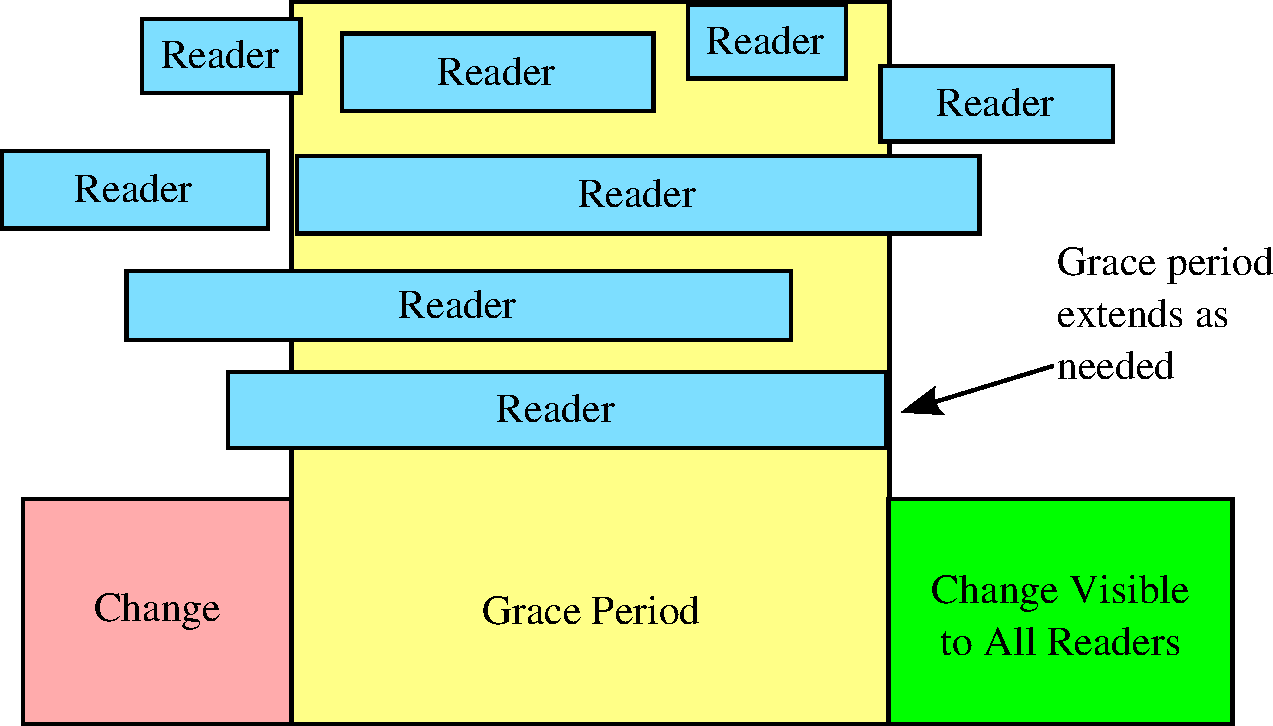
\includegraphics[scale=0.35]{rcu_concepts.pdf}
\caption{Поведение RCU}
\label{fig:rcu_concepts}
\end{figure}

\subsection{Программный интерфейс RCU} \label{sec:api_usage}
Программный интерфейс RCU достаточно невелик и состоит всего из пяти операций:
\co{rcu_read_lock()}, \co{rcu_read_unlock()}, \co{synchronize_rcu()},
\co{rcu_assign_pointer()}, and \co{rcu_dereference()}~\cite{McKenneyOSR08}.

Критическая секция RCU-читателя начинается с \co{rcu_read_lock()}
и заканчивается соответсвующим \co{rcu_read_unlock()}.
Вложенные критические секции чтения объединяются.
Внутри критической секции запрещается блокирование данного потока.
Данные, чтение которых осуществляется доступ внутри критической секции RCU,
будут доступны до её окончания.

Функция \co{synchronize_rcu()} соответсвует окончанию выполнения кода,
обновляющего значение объекта, тем самым сигнализируя о начале фазы освобождения.
Она блокирует поток-писатель до тех пор, пока все потоки-читатели
не выйдут из своих критических RCU-секций.
Отметим, что \co{synchronize_rcu()} не ожидает окончания
критических секций, вход в которые был осуществлен позже её вызова.

%\comment{Lihao: add example, e.g. http://paulmck.livejournal.com/39343.html}

\begin{figure}[tbp]
\centering
\footnotesize
\begin{verbatim}
               int x = 0;
               int y = 0;
               int r1, r2;

               void rcu_reader(void) {
                 rcu_read_lock();
                 r1 = x;
                 r2 = y;
                 rcu_read_unlock();
               }

               void rcu_updater(void) {
                 x = 1;
                 synchronize_rcu();
                 y = 1;
               }

               ...

               // after both rcu_reader()
               // and rcu_updater() return
               assert(r2 == 0 || r1 == 1);
\end{verbatim}
\caption{Verifying RCU Grace Periods}
\label{fig:verify_rcu_gp}
\end{figure}

Рассмотрим пример, приведенный на рисунке~\ref{fig:verify_rcu_gp}.
Если вход в критическую секцию чтения функции \co{rcu_reader()} выполнится до
вызова \co{synchronize_rcu()} в \co{rcu_updater()}, то выход из ней должен быть
совершен до возврата из \co{synchronize_rcu()}, чтобы значение переменной
\co{r2} было равно 0. Если же вход в неё произойдет после возврата из
\co{synchronize_rcu()}, то значение \co{r1} будет равным 1.

Наконец, для присвоения нового значения указателю, защищенному RCU,
потоки-писатели должны использовать \co{rcu_assign_pointer()},
которая возвращает новое значение.
RCU-читатели могут использовать \co{rcu_dereference()} для чтения
указателя, защищенного RCU, который впоследствии может быть безопасно разыменован.
%Note that this API does not actually dereference the pointer.
%Instead, it only fetches the pointer for later dereferencing.
Возвращаемое ею значение является корректным лишь внутри критической секции.
% Lihao: include this in PhD thesis and the technical report
Функции \co{rcu_assign_pointer()} и \co{rcu_dereference()} используются в паре
для того, чтобы убедиться, что если данный поток-читатель разыменовывает
защищенный указатель на только что вставленный объект, операция разыменования
вернет корректное значение, а не недоинициализированный мусор.

